\section{R\'enyi, Tsallis and mixed-state entropies}\label{sec:fqe-spectral}

Different spectral entropies give different weights to the marginal eigenvalues. For $q>0$, $q\ne1$, the R\'enyi~\cite{Renyi} and Tsallis~\cite{Tsallis} entropies
\[
 H_q(\rho)=\frac{\log_2\operatorname{tr}\rho^q}{1-q},\qquad
 S_q(\rho)=\frac{1-\operatorname{tr}\rho^q}{q-1}
\]
tend as $q\to1$ to $S(\rho)$ in bits and $(\ln2)S(\rho)$ in nats,
respectively. As $q\to0$, $H_q$ tends to the base-two logarithm of the rank of $\rho$, which is the Schmidt rank across a pure-state cut; $H_2=-\log_2\operatorname{tr}\rho^2$ is fixed by the
purity, the quantity minimised at seven qubits and the one that randomised-measurement experiments estimate
directly~\cite{Brydges19}; as $q\to\infty$, $H_q$ depends only on the largest eigenvalue. Each is Schur-concave: averaging any pair of eigenvalues cannot lower it. For
pure states it therefore does not increase under deterministic local operations and classical communication~\cite{Nielsen99}:
every member measures how entangled a cut is. Asking which state maximises them all tests whether ``most entangled''
is a robust notion. The answer depends on the order: $M_4$ maximises the mean R\'enyi entropy for $q<q_*\approx1.588$, and the cluster states maximise it for $q>q_*$. For the Tsallis entropies $M_4$ is the maximiser for $0<q<2$; the cluster states tie with it at $q=2$ and beat it for every $q>2$. The
maximiser for $q>2$ is identified by Gour and Wallach~\cite[Theorem~9(a)]{GW}; we do not reprove that result. The cut spectra explain the change. Those of the cluster state are
flat, $(\tfrac12,\tfrac12)$ on one cut and uniform $\tfrac14$ on the other two, so its mean R\'enyi entropy is $5/3$ for
every $q$; the lopsided spectrum $(\tfrac12,\tfrac16,\tfrac16,\tfrac16)$ of $M_4$ gives a mean $H_q$ falling from
$2$ bits as $q\to0$ to $1$ bit as $q\to\infty$. Small $q$ favours full rank and large $q$ a small largest
eigenvalue, hence the crossing at $q_*$. The Tsallis tie at $q=2$ holds because $1-\operatorname{tr}\rho^2$ depends
only on the cut purities, and both states have $P=1$.

The cubic-majorant argument applies to a wider class of spectral functionals. We state that criterion and
apply it to Tsallis entropies and R\'enyi orders below one; orders above one need additional estimates
(Appendix~\ref{sec:fqe-renyi-proofs}). We then transfer the pure-state bounds to mixed-state convex roofs. We retain
the notation \(P,T,F,\tau\) from the maximum proof; proofs not given here are in Appendix~\ref{sec:fqe-spectral-proofs}.

\begin{proposition}[Cubic spectral majorants]\label{prop:fqe-majorant}
For continuous $f:[0,1]\to\mathbb R$, set
\[
\mathcal E_f(\psi)=\frac13\sum_{j=2}^4\operatorname{tr}f(\rho_{1j}).
\]
Suppose $h(x)=ax^3+bx^2+cx+d$ majorises $f$ on $[0,1]$, agrees with $f$
at $1/6$ and $1/2$, and satisfies $a\ge0$, $b+17a/12\le0$.
Then $\mathcal E_f(\psi)\le\mathcal E_f(M_4)$ for every pure four-qubit state.
If both coefficient inequalities are strict, equality holds precisely on the two HS LU orbits.
\end{proposition}
\begin{proof}
Put $\alpha=-b-17a/12$ and
$\Delta_f=\sum_{j,\lambda\in\operatorname{spec}\rho_{1j}}(h-f)(\lambda)\ge0$.
Summing the cubic and subtracting its value at $M_4$ gives
\[
3\bigl(\mathcal E_f(M_4)-\mathcal E_f(\psi)\bigr)
=\alpha(P-1)+\frac a{12}F+\Delta_f.\tag{SF}\label{eq:fqe-spectral}
\]
All three terms are nonnegative, since $P\ge1$ (Lemma~\ref{lem:fqe-purity}) and $F\ge0$
(Theorem~\ref{thm:fqe-moment}). The same two nonnegative moment defects therefore control every functional
satisfying the coefficient conditions. If $a,\alpha>0$, equality requires $P=1$ and $F=0$,
so Proposition~\ref{prop:fqe-moment-zeros} gives the HS orbits; the other zeros of $F$, the products of two Bell pairs,
have $P=3/2$ and are excluded. No strict scalar
majorisation is required. For differentiable $f$, a candidate touching cubic
is its Hermite interpolant at the two nodes.
\end{proof}

\begin{corollary}[Tsallis entropies]\label{cor:fqe-tsallis} For every \(0<q<2\), \(q\ne1\), the mean
Tsallis-\(q\) entropy of the three cuts satisfies \[
\boxed{\quad
\tfrac13\sum_{j=2}^4\frac{1-\operatorname{tr}\rho_{1j}^q}{q-1}
\ \le\ \frac{1-2^{-q}-3\,6^{-q}}{q-1}\quad}
\] with equality iff \(\psi\) is LU-equivalent to \(M_4\) or \(\overline{M_4}\). \end{corollary}
The range is sharp: at \(q=2\) equality is no longer unique, and for every \(q>2\) the cluster state beats \(M_4\)
(proved in Appendix~\ref{sec:fqe-spectral-proofs}, which also gives the corresponding quadratic deficit bounds).

\paragraph{R\'enyi entropies.} With $H_q$ as above, write
\[
\mathcal E_q(\psi)=\frac13\sum_{j=2}^4H_q(\rho_{1j}),\qquad
h_q=\mathcal E_q(M_4)=\frac{\log_2(2^{-q}+3\,6^{-q})}{1-q}.
\]
At $q=1$ these have their continuous von Neumann values in bits.

\begin{corollary}[R\'enyi entropies below one]\label{cor:fqe-renyi} For \(0<q<1\), concavity of
\(\log\) and the Tsallis bound imply \[
\frac13\sum_{j=2}^4
\frac{\log_2\operatorname{tr}\rho_{1j}^q}{1-q}
\le \frac{\log_2(2^{-q}+3\,6^{-q})}{1-q},
\] again with exactly the same LU equality classes. The argument does not assert the analogous R\'enyi
bound for \(q>1\).

\end{corollary}
\noindent Equality needs equality in the Tsallis bound, hence the HS orbits, and in Jensen's inequality for the logarithm
over the three cuts, which holds there because the three cuts of $M_4$ have identical spectra.

Orders above one require additional estimates. The full result is as follows, with $q_*$ the
unique order for which $h_{q_*}=5/3$ (Proposition~\ref{prop:fqe-renyi-crossing}).

\begin{corollary}[R\'enyi envelope of Gour and Wallach]\label{cor:fqe-renyi-gw}
For every pure four-qubit state and every $q>0$, $\mathcal E_q(\psi)\le\max\{h_q,5/3\}$.
For $q<q_*$ the maximisers are exactly the two HS LU orbits;
for $q>q_*$ they are the cluster states up to local unitaries and qubit permutations (every permutation of the three cuts is induced by a permutation of the qubits).
At $q=q_*$ both classes, and only those classes, attain the bound.
\end{corollary}
Below one the bound follows from the preceding corollary, and at $q=1$ from
Theorem~\ref{thm:fqe-entropy-max}. For $q>1$ it is proved in Appendix~\ref{sec:fqe-renyi-proofs}, which opens with a
plan of the argument; for $1<q<2$ the proof is analytic apart from exact finite checks, namely an exact six-copy
certificate bounding the variance of the three cut purities and exact polynomial sign checks.
Figure~\ref{fig:fqe-renyi} shows the change of maximiser.

\begin{figure}[t]
\centering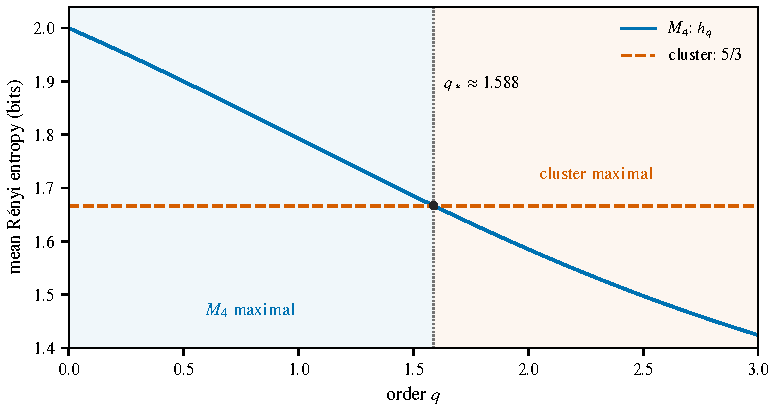
\includegraphics[width=0.8\linewidth]{fig_renyi}
\caption{Change of R\'enyi-entropy maximiser with the order $q$. The mean entropy of $M_4$
($h_q$, solid) and that of the cluster states ($5/3$, dashed) cross once, at $q_*\approx1.588$
(Proposition~\ref{prop:fqe-renyi-crossing}). The larger of the two, $\max\{h_q,5/3\}$,
is the maximum over all pure four-qubit states (Corollary~\ref{cor:fqe-renyi-gw}):
$M_4$ attains it below $q_*$ and the cluster states above $q_*$ (shaded regions). Values at $q=0$ and $q=1$
are continuous limits.}
\label{fig:fqe-renyi}
\end{figure}

\subsection{Mixed-state entanglement}\label{sec:fqe-spectral_corollaries-mixed-state-entanglement}

For a mixed state, the entropy of a marginal also counts classical mixing, which is not entanglement: the
maximally mixed four-qubit state has maximally mixed marginals but no entanglement. We therefore use the
\emph{convex roof}: the least average of a pure-state spectral functional over all ensembles representing the state,
as in the entanglement of formation~\cite{BDSW}.
For a general $f$ obeying the hypotheses below, this construction is an entanglement
monotone when the induced function of the marginal is concave and vanishes on pure marginals, as for the von
Neumann and Tsallis entropies; the ceiling below needs neither property.
In the cut notation below, $\widehat{1j}$ denotes the complementary pair.

\begin{corollary}[Convex roofs]\label{cor:fqe-convex-roof} Let \(f\) satisfy the hypotheses of
Proposition~\ref{prop:fqe-majorant}. For each cut define the convex roof \[
E_f^{1j|\widehat{1j}}(\rho)=
\inf_{\rho=\sum_\ell p_\ell|\psi_\ell\rangle\langle\psi_\ell|}
\sum_\ell p_\ell\operatorname{tr}f(\rho_{1j}^{(\ell)}).
\] Then every mixed four-qubit state satisfies \[
\frac13\sum_{j=2}^4 E_f^{1j|\widehat{1j}}(\rho)
\le\mathcal E_f(M_4).
\] If both coefficient inequalities of Proposition~\ref{prop:fqe-majorant} are strict, equality holds exactly
for pure states in the two \(M_4\) LU orbits. For \(f=-x\log_2x\) these are the three bipartite
entanglements of formation. The same HS ceiling and pure-only equality classification hold for
the Tsallis entropies with $0<q<2$ and the R\'enyi entropies with $0<q<q_*$, including their
von Neumann limits at $q=1$.

\end{corollary}
To prove the ceiling, fix any pure-state ensemble $\rho=\sum_\ell p_\ell|\psi_\ell\rangle\langle\psi_\ell|$.
Each cut's roof is at most that cut's ensemble average, so the mean of the three roofs is at most
$\sum_\ell p_\ell\,\mathcal E_f(\psi_\ell)\le\mathcal E_f(M_4)$ by Proposition~\ref{prop:fqe-majorant} (in the R\'enyi case, with
$\mathcal E_q$ in place of $\mathcal E_f$, by Corollary~\ref{cor:fqe-renyi-gw}). Appendix~\ref{sec:fqe-spectral-proofs} excludes mixed maximisers:
every mixed-state support contains a vector of deficient Schmidt rank (fewer than four nonzero Schmidt coefficients
across a given $2|2$ cut), whereas every pure maximiser has full rank there.
